The goal of this assignment is to design and implement a network-based application that provides real-time monitoring and communication functionalities. The system must support node-to-node interaction, dynamic data handling, and practical deployment in a real-world environment.

\subsection{HydroTracker}

\textit{HydroTracker} is a smart service-assistance system designed for use in cafés and similar settings. Its core concept is based on a distributed network of coaster-shaped sensing nodes that monitor water glass levels.

Each coaster node integrates a load cell — a force sensor that varies resistance with applied weight — connected to an Arduino Uno microcontroller. These microcontrollers act as \textbf{transmitters}, processing the weight data locally and sending it wirelessly to a central \textbf{receiver node}, also built on an Arduino. The receiver collects the measurements from all transmitters and forwards them via serial communication to a host computer. There, a data processing application interprets the input and presents it in a graphical user interface, clearly displaying the fill level of each glass using intuitive color indicators.

\begin{figure}[H]
    \centering
    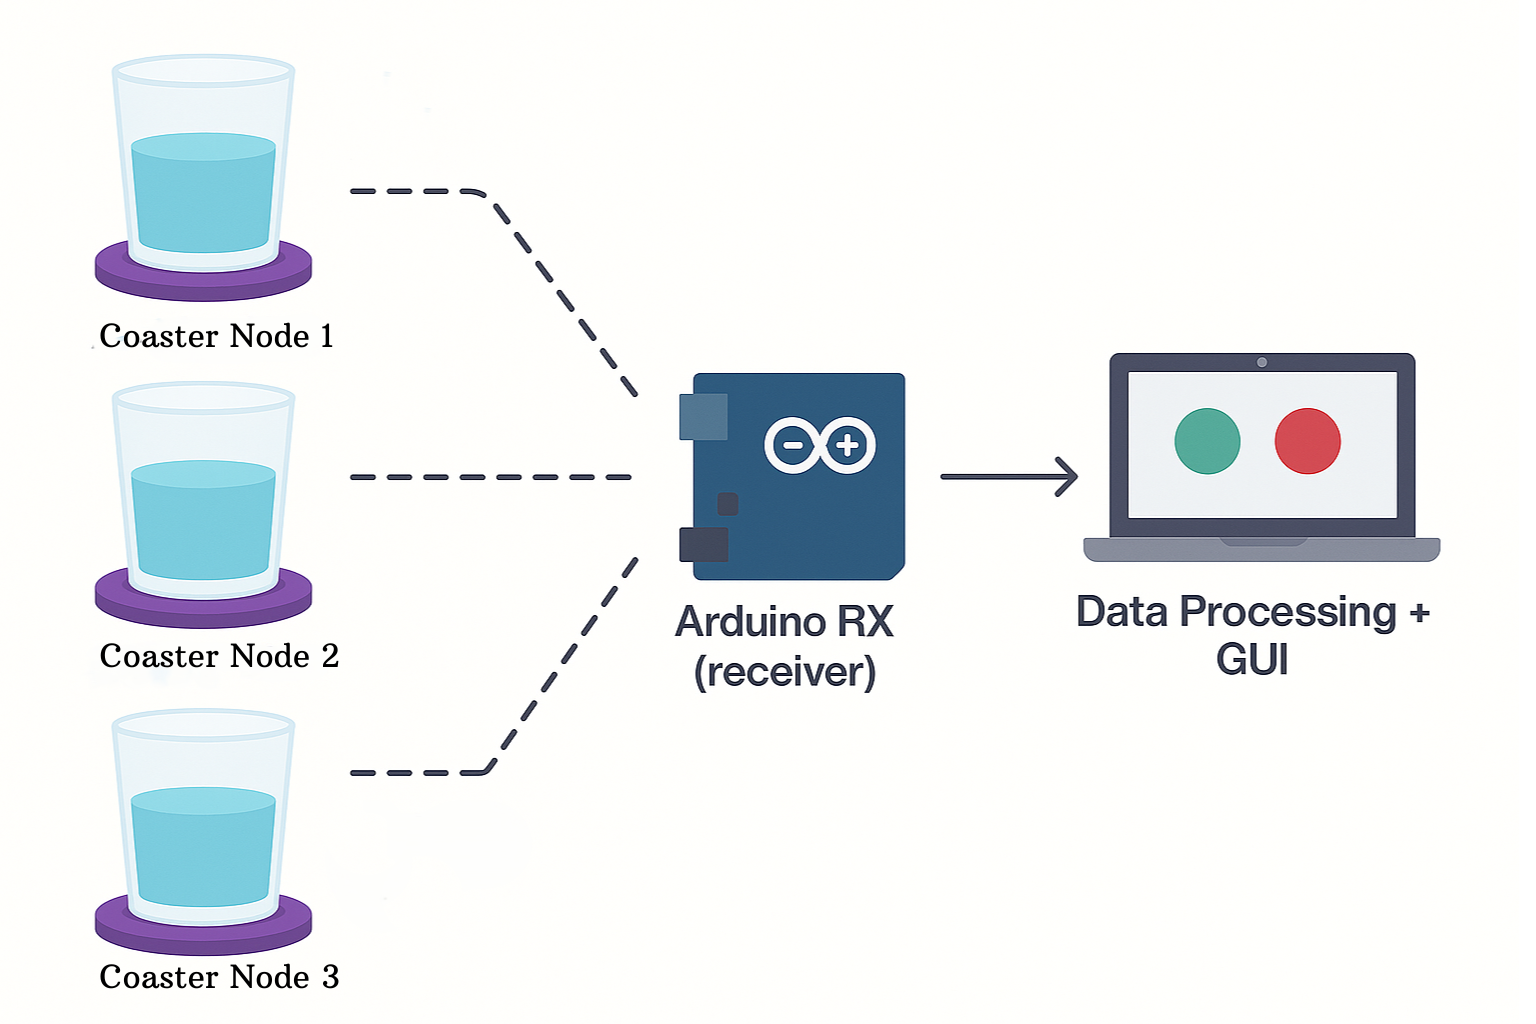
\includegraphics[width=0.5\linewidth]{gui_images/Arduino TX.png}
  \caption{HydroTracker system architecture}
  \label{fig:hydrotracker_architecture}
\end{figure}

The main purpose of HydroTracker is to help waitstaff monitor tables efficiently, without having to constantly check every glass manually. This reduces unnecessary effort, streamlines service flow, and enhances the overall customer experience. Additionally, thanks to its modular and scalable architecture, HydroTracker can be extended beyond cafés—such as into office spaces, hospitals, or coworking environments—offering smart hydration tracking wherever needed.